\documentclass{article}

\usepackage{graphicx}
% if you need to pass options to natbib, use, e.g.:
%     \PassOptionsToPackage{numbers, compress}{natbib}
% before loading neurips_2023


% ready for submission
%\usepackage{neurips_2023}


% to compile a preprint version, e.g., for submission to arXiv, add add the
% [preprint] option:
\usepackage[preprint]{neurips_2023}


% to compile a camera-ready version, add the [final] option, e.g.:
%     \usepackage[final]{neurips_2023}


% to avoid loading the natbib package, add option nonatbib:
%    \usepackage[nonatbib]{neurips_2023}


\usepackage[utf8]{inputenc} % allow utf-8 input
\usepackage[T1]{fontenc}    % use 8-bit T1 fonts
\usepackage{hyperref}       % hyperlinks
\usepackage{url}            % simple URL typesetting
\usepackage{booktabs}       % professional-quality tables
\usepackage{amsfonts}       % blackboard math symbols
\usepackage{nicefrac}       % compact symbols for 1/2, etc.
\usepackage{microtype}      % microtypography
\usepackage{xcolor}         % colors


\title{Myers Briggs personality predicting}


% The \author macro works with any number of authors. There are two commands
% used to separate the names and addresses of multiple authors: \And and \AND.
%
% Using \And between authors leaves it to LaTeX to determine where to break the
% lines. Using \AND forces a line break at that point. So, if LaTeX puts 3 of 4
% authors names on the first line, and the last on the second line, try using
% \AND instead of \And before the third author name.


\author{
  %
  Matthew Rogers \thanks{Use footnote for providing further information
    about author (webpage, alternative address)---\emph{not} for acknowledging
    funding agencies.} \\
  School of Computing\\
  Clemson University\\
  %
  \texttt{mwr2@clemson.edu} \\
  % examples of more authors
  \And
  Yue Zhang\\
  School of Computing\\
  Clemson University\\
  % Coauthor \\
  % Affiliation \\
  % Address \\
  \texttt{yzhng@clemson.edu} \\
  % \AND
  % Coauthor \\
  % Affiliation \\
  % Address \\
  % \texttt{email} \\
  % \And
  % Coauthor \\
  % Affiliation \\
  % Address \\
  % \texttt{email} \\
  % \And
  % Coauthor \\
  % Affiliation \\
  % Address \\
  % \texttt{email} \\
}


\begin{document}


\maketitle


\begin{abstract}
  The Myers Briggs personality assessment puts a personality type to an individual. There are four components to an individual’s personality. For each component, an individual takes on one out of two attributes. Since each of the four components has two attributes, then there are sixteen different personality types that an individual can be labeled as. For the first component there is introversion vs. extroversion, for the second there is intuition vs. sensing, for the third thinking vs feeling, and for the last component there is judgment vs perception. The objective of this project is to investigate the effectiveness of the perceptron to label each component of an individual’s personality type.
 
\end{abstract}


\section{Introduction}
The purpose of this project was to investigate the efficiency of different classification models to predict the personality type of an individual based on twitter posts. The motivation of exploring this subject is this research can help companies to provide personalized services and recommendations based on one’s personality preferences and needs and this research can also help social media sites enhance a user’s presence and reputation by choosing the most suitable posts and interactions. The dataset used in the research included 6940 anonymous individuals, each labeled with a Myers Briggs personality type. Each individual had a series of twitter posts associated with them. To help in the classification of the individual’s personality linear, polynomial, sigmoid, and gaussian radial basis SVM, and perceptron were used.
The Myers-Briggs personality type is a way to label individual with a certain personality. This personality type is made up of 4 personality trait pairs. The first is introversion vs extroversion. This pair is the measure of an individual’s preference for the inner or outer world.
 	The second pair is intuition vs sensing are the information gathering functions. They describe how new information is gathered and interpreted. People who prefer sensing are more likely to trust information in the present, tangible, and concrete. People who prefer intuition tend to trust information that can be associated with other information.	
	The third pair is thinking vs feeling. These are the decision-making functions. Those who prefer thinking tend to decide things from a more detached standpoint, measuring the decision what seems logical, reasonable, causal, consistent, and matching a given set of rules. Those who prefer feeling tend to come to decisions based on associating or empathizing with the situation.
	The fourth pair is judging vs perceiving. Judging refers to whether an individual displays their thinking or feeling function whereas perceiving refers to whether an individual displays their intuition or sensing function. 

\section{Background}

Due to the nature of the Myers-Briggs type , we can break down the classification task with 16 classes in to 4 binary classification tasks. This is because a MBTI type is composed of 4 binary classes, where each binary class represents a dimension of personality of the MBTI personality model as theorized by the inventors. Therefore, instead of training a multi-class classifier, we instead train 4 different binary classifiers, such that each specializes in one of the dimensions of personality. 

Once these new datasets were produced, each dataset (each one was a csv file) was transformed into a table in MATLAB. The rows were sorted on the attribute column so that one type would appear first before the other one. For example, if the dataset with the first attribute was being used, then each individual labeled as an introvert would appear first and then the individuals labeled as extroverts would appear second. Then, a certain number of rows for each type were taken and were combined to form a training set. The other rows remaining were combined to form the test set. After each set was randomly permutated and standardized (the zscore function was used), training set was put through a linear perceptron algorithm to find the weights. Using these weights, the test set was put through another algorithm to test the accuracy of this perceptron. 
\section{Methods}
\subsection{Preprocessing}
When we examined other studies of MBTI using machine learning, we were surprised to find that researchers rarely made a point of cleaning their data set to accord with the actual proportions of MBTI types in the general population (e.g. ISTJ = 0.11, ISFJ = 0.09, etc.)[3]. Since our raw data set is severely disproportional (see fig. 1) compared to the roughly uniform distribution for the general population, it was clear to us that some cleaning of the proportional representation of each MBTI type would be necessary. Therefore, we artificially made our test set reflect the proportions found for each type in the general population, so as to prevent any misinterpretation of results due to skewed representation of classes in the test set.
\begin{figure}
  \centering
  \fbox{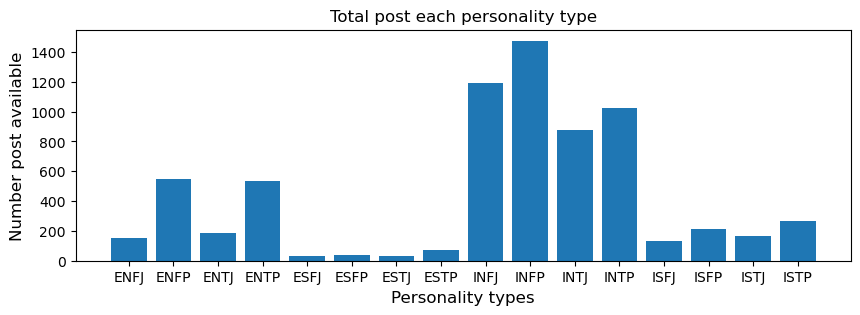
\includegraphics[width=1.\linewidth]{1.png}}
  \caption{ Distribution of MBTI types in the data set.}
\end{figure}
% \subsection{Style}
\subsubsection{Meaningless words removal}
As the dataset is sourced from an online forum where communication is solely through written text, certain modifications were necessary. Notably, instances of data points containing hyperlinks were eliminated, aiming to foster the model's generalization to the English language. Additionally, to enhance the meaningfulness of each word in the dataset, so-called "stop words," such as common fillers like "a," "the," "or," etc., were excluded using the NLTK library in Python. Lastly, considering the dataset's origin from a website dedicated to explicit discussions about personality models, particularly MBTI, references to specific types (e.g., 'INTJ,' 'INFP,' etc.) were expunged. This measure was taken to prevent the model from potentially "cheating" by learning to recognize MBTI mentions explicitly by name.
\subsubsection{Transfer to root words}
To transfer to root words on the text, 
we employed the nltk.stem.WordNetLemmatizer. 
This process involved transforming inflected forms of the same root word into their dictionary form; for instance, "walking," "walked," and "walk" were all lemmatized to "walk." This approach enables us to capitalize on the shared meaning inherent in various inflected forms of a given word.
\begin{figure}
  \centering
  \fbox{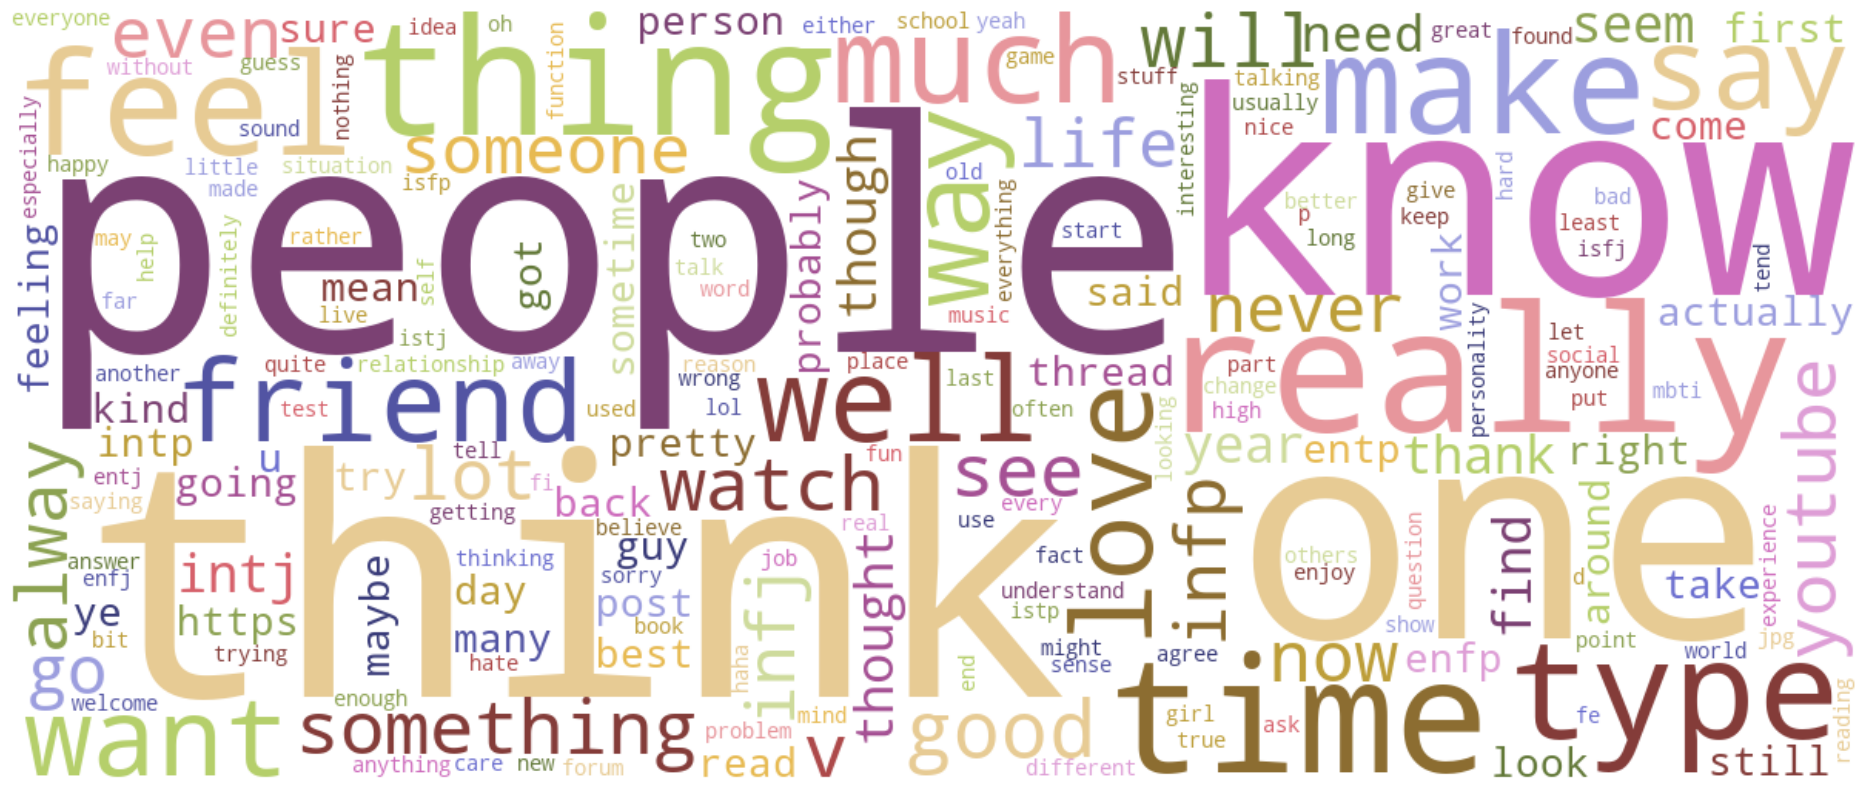
\includegraphics[width=.5\linewidth]{before.png}}
  \caption{ Before Preprocessing.}
\end{figure}
\begin{figure}
  \centering
  \fbox{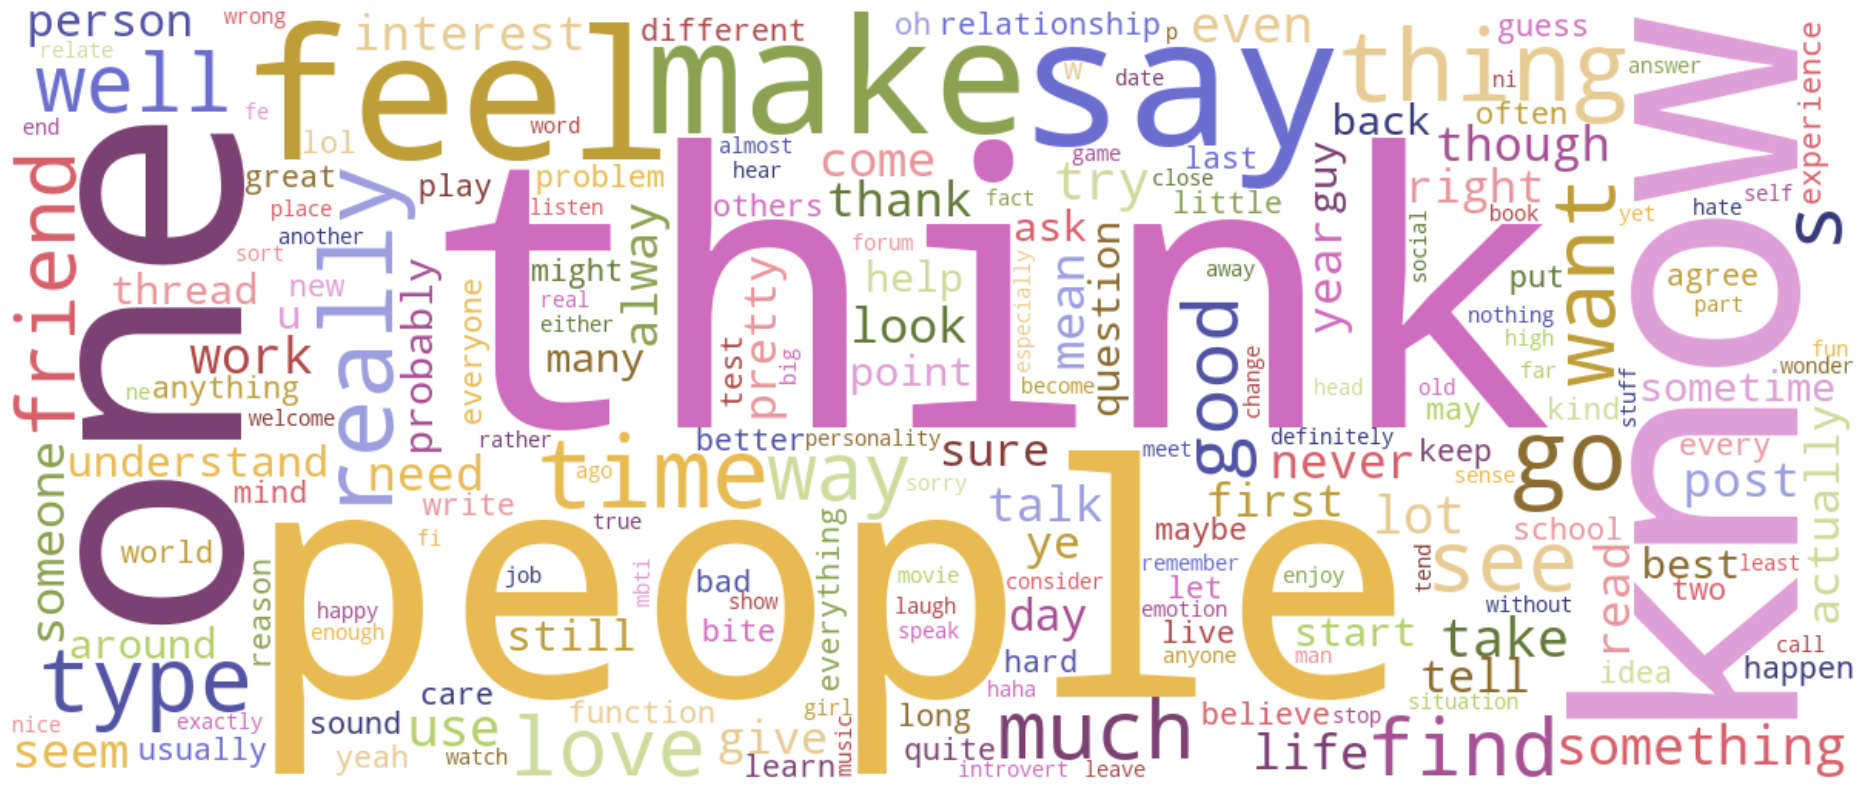
\includegraphics[width=.5\linewidth]{after.png}}
  \caption{ After Preprocessing.}
\end{figure}
\subsubsection{Input format}
First, we picked up 500 most commom words from the proprocessed dataset,
\\
('think', 39658),('get', 28446),('people', 27788),('know', 24659),('one', 21477),('feel', 21454),.....

Then we build a vector of 500 elements to represent each post which each element is the frequency of these 500 words in the post.
\begin{equation}
 [f_0,f_1,...,f_{499}]^T
\end{equation}

\subsection{Dimesion removal}
To prevent overfitting and enhance efficiency, we have decided to attempt using PCA for data dimensionality reduction.
To determine the appropriate number of dimensions, we created a figure in which 
The x-axis represents the number of selected dimensions, and the y-axis represents the percentage of information represented after selecting the current number of dimensions.
\begin{figure}
  \centering
  \fbox{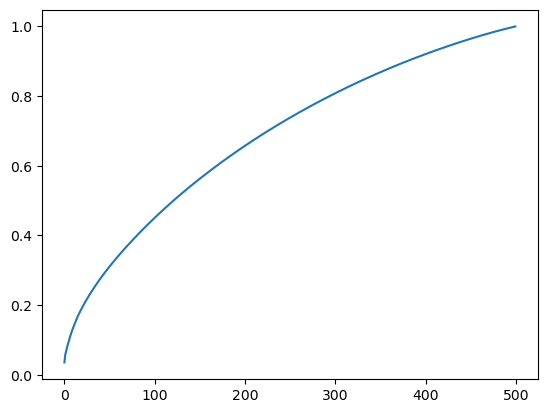
\includegraphics[width=.4\linewidth]{pca.png}}
  \caption{ dimension vs percentage of info..}
\end{figure}
from the figure, we couldn't find a turning point where there is sufficient information at the point. Beyond this point, there is no significant increase in the amount of information
In summary, we are unable to perform dimensionality reduction on the data.

\subsection{SVM}
The final dual formulation of kernel svm can be represented by 
\begin{equation}
  \max_\lambda-\frac{1}{2}\sum_i\sum_j\lambda_i\lambda_jy_iy_jK(x_i,x_j)
\end{equation}
We tried 4 different kernels in our project, they are
\begin{itemize}
  \item linear: $K(x,y) = x^Ty$
  \item poly: $K(x,y) = (\gamma (x^Ty)+r)^d$
  \item sigmoid: $K(x,y) = tanh((x^Ty)+r)$
  \item  $K(x,y) = e^{-\gamma ||x-y||^2}, \gamma>0$
\end{itemize}
Also, we test different values for the penalty term $C$ in the original problem
\begin{equation}
  \min_{\omega,b,\epsilon} \frac{1}{2}\omega^T\omega + C\sum_i^n\epsilon_i
\end{equation} 
\section{Resuts}
\subsection{All attributes}

see Table [\ref{all}]
\begin{table}
  \caption{All attributes}
  \label{all}
  \centering
  \begin{tabular}{llll}
    \toprule
    \cmidrule(r){1-2}
    Kernel     & Train Accuracy   & Time consumption  & Test Accuracy  \\
    \midrule
    RBF & 0.734047  & 30.857661 &   0.317003   \\
    Poly     & 0.987855 & 35.146751 &  0.316042    \\
    Linear     & 0.475504	& 25.300210      & 0.310279  \\
    Sigmoif & 0.365377 & 25.245560 & 0.306916\\
    \bottomrule
  \end{tabular}
\end{table}

\subsection{Extraversion vs. Introversion}
see Table [\ref{IE}]

\begin{table}
  \caption{IE}
  \label{IE}
  \centering
  \begin{tabular}{llll}
    \toprule
    \cmidrule(r){1-2}
    Kernel     & Train Accuracy   & Time consumption  & Test Accuracy  \\
    \midrule
    RBF & 0.838617  & 24.255259 &   0.770893   \\
    Poly     & 0.991149 & 26.795339 &  0.769933    \\
    Linear     & 0.770893	& 16.092506      & 0.770413  \\
    Sigmoif & 0.757102 & 7.945040 & 0.770413\\
    \bottomrule
  \end{tabular}
\end{table}
\subsection{Sensing  vs. Intuition }

see Table [\ref{NS}]

\begin{table}
  \caption{NS}
  \label{NS}
  \centering
  \begin{tabular}{llll}
    \toprule
    \cmidrule(r){1-2}
    Kernel     & Train Accuracy   & Time consumption  & Test Accuracy  \\
    \midrule
    RBF & 0.870111  & 21.805165 &   0.770413   \\
    Poly     & 0.998353 & 23.301729 &  0.768012    \\
    Linear     & 0.862907	& 13.397481      & 0.770413  \\
    Sigmoif & 0.862495 & 6.643756 & 0.770413\\
    \bottomrule
  \end{tabular}
\end{table}

\subsection{Thinking  vs. Feeling }
see Table [\ref{TF}]

\begin{table}
  \caption{TF}
  \label{TF}
  \centering
  \begin{tabular}{llll}
    \toprule
    \cmidrule(r){1-2}
    Kernel     & Train Accuracy   & Time consumption  & Test Accuracy  \\
    \midrule
    RBF & 0.931247	  & 23.654586 &   0.710855   \\
    Poly     & 0.994648 & 28.503457 &  0.695485    \\
    Linear     & 0.782627	& 13.486006      & 0.709414  \\
    Sigmoif & 0.695760 & 16.708707 & 0.695965\\
    \bottomrule
  \end{tabular}
\end{table}

\subsection{Judging  vs. Perceiving }

see Table [\ref{JP}]

\begin{table}
  \caption{JP}
  \label{JP}
  \centering
  \begin{tabular}{llll}
    \toprule
    \cmidrule(r){1-2}
    Kernel     & Train Accuracy   & Time consumption  & Test Accuracy  \\
    \midrule
    RBF & 0.898312	  & 25.711215 &   0.645053  \\
    Poly     & 0.994236 & 31.332261 &  0.645053    \\
    Linear     & 0.703993	& 14.384366      & 0.643132  \\
    Sigmoif & 0.611980 & 15.768533 & 0.640250\\
    \bottomrule
  \end{tabular}
\end{table}

\subsection{different penalty term on linear kernel}
we also tried different $C$ from 0 to 1 to improve the accuracy, see figure \ref{fig:C}
\begin{figure}
  
  \centering
  \fbox{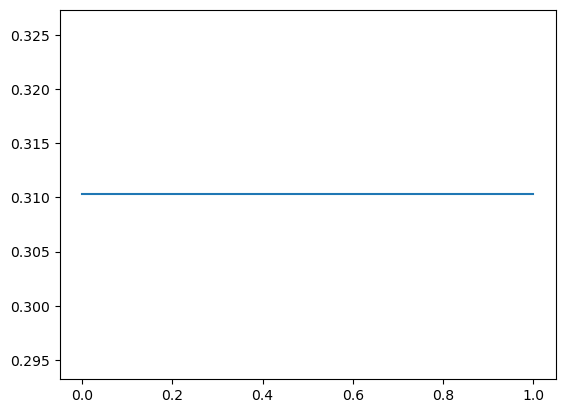
\includegraphics[width=.4\linewidth]{c.png}}
  \caption{ C value vs. Accuracy}
  \label{fig:C}
\end{figure} 
\subsection{Conclusion}
SVMs are not performing very well on this job

\section{Based on letters}
As mentioned in the proposal, for each row (anonymous individual) there was a personality type made up of four attributes and a certain number of columns with each column containing a whole or part of a twitter post. The first objective was to combine all these columns into one so that there was just one column containing all the posts for each individual. The second objective was to split up the personality type into four separate columns where each column represented an attribute. For example, if an individual was labeled as IFSP, then this column would be split into four attributes where the first attribute would be labeled as I, the second attribute labeled as F, etc. These transformations were done in Excel.\\
For the first part of our research project, it wanted to be determined if there was an association between the average of different letters and the individual’s specific attribute type. To see if there was an association, the frequency of each letter was found for each row (individual). Since, each individual varied on the number of letters used for all of their posts, the average was then calculated for each letter frequency. For example, if an individual used a total of 20000 characters and used the letter ‘a’ in 1000 instances, then there would be a score of .05 (instances/ total \# of characters). After, the average was calculated for each letter for each individual, then this new dataset was split into four datasets where each dataset concentrated on a specific attribute (I vs E, F vs T, etc.). This part of the project was done in Python.
\\
After using this process for each dataset and varying the number of entries in the training set and varying the number of iterations the perceptron took to find the weights, it was observed the accuracy varied significantly. Accuracy scores approximately ranged from 35\% to 70\%. It was questioned whether perhaps the specific sample used could explain these observations. In other words, maybe choosing an appropriate training set could make the perceptron more accurate by being more representative of the rest of the dataset.
\\
A clustering approach in Python was used to investigate this question. Specifically, Kmeans was used from the Sci-kit Learn package. The intent of the overall process about to be outlined was to cluster the whole population (all the entries in a particular dataset) into groups based on a mean value. Then, a representative would be chosen from each group to be used for the training set. Perhaps, this representative training sample could lead to a higher accuracy score using the linear perceptron.
\\
The specific process started with using just one dataset with the second attribute (F vs T). The columns that were not going to be used in the clustering algorithm were dropped. The data frame was then grouped by the binary classification (1 or -1) and then was split into two separate data frames based on this classification. 
\\
Kmeans was then used for each dataset with a certain number of means (but the same) to cluster both data frames. After adding a cluster group column in each data frame, each row (in each data frame) was labeled with its corresponding group number. Each data frame, was then sorted in ascending order based on its cluster group number. A representative was then chosen from each group from each data frame. This representative was chosen by being first the first entry for each group. All the representatives were then put into a training set and the rest of the entries were put in a test set. Each set was then randomly permutated and the cluster group column was dropped. The training and test set were then converted to an array so that it was an acceptable form to be used by the linear perceptron model from the Sci-kit Learn package. The training set was used to train this model and then the test set was used to measure its accuracy.

\subsection{letters result}
See figure\ref{fig:letter}\\
The accuracy was measured using a different number of training ‘representatives’. This number was only changed a few times (so there were only a few accuracy scores) but the accuracy did not get above 55\%. This process was rudimentary since it did not find the ‘best’ representative of the group. In other words, it did not find the group member with the lowest average mean. At this time, it is also uncertain how 70\% was even achieved in the initial perceptron process (MATLAB). These questions still need to be investigated. However, it was concluded that looking at frequency averages of letters did not provide a significant way of labeling each attribute. Therefore, the next portion of the project was dedicated to investigating the words used instead of the frequency averages of the letters.

\begin{figure}
  
  \centering
  \fbox{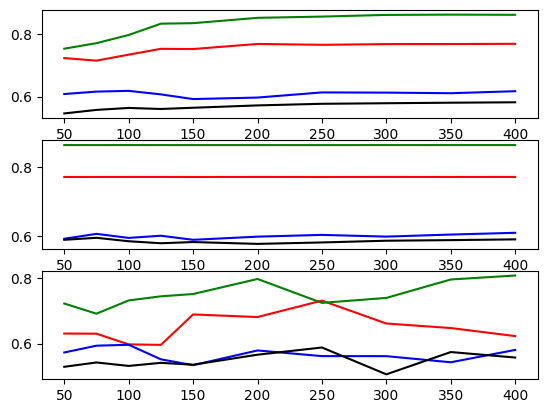
\includegraphics[width=.5\linewidth]{letter.png}}
  \caption{ for each attribute}
  \label{fig:letter}
\end{figure} 

\subsection{Observation \& conclusion}
The accuracy is misleading:
\begin{itemize}
  \item Consider the trait pair with highest accuracy (N/S)
  \item There were 5988 N’s and 952 S’s
  \item Algorithm could have guessed N for all samples
  \item Accuracy $= 5988/6940 = 86.2\%$
\end{itemize}
Similarly, if algorithm guessed ‘dominant’ trait for other sets:
\begin{itemize}
  \item $I\/E \rightarrow 77.1\%$
  \item $T\/F \rightarrow 54.5\%$
  \item $P\/J \rightarrow 60.2\%$
\end{itemize}

Therefore, it was concluded that the kernel svm model and the other classification models were NOT accurate in predicting personality traits based on letter frequency average

% Please read the instructions below carefully and follow them faithfully. \textbf{Important:} This year the checklist will be submitted separately from the main paper in OpenReview, please review it well ahead of the submission deadline: \url{https://neurips.cc/public/guides/PaperChecklist}.




% Papers to be submitted to NeurIPS 2023 must be prepared according to the
% instructions presented here. Papers may only be up to {\bf nine} pages long,
% including figures. Additional pages \emph{containing only acknowledgments and
% references} are allowed. Papers that exceed the page limit will not be
% reviewed, or in any other way considered for presentation at the conference.


% The margins in 2023 are the same as those in previous years.


% Authors are required to use the NeurIPS \LaTeX{} style files obtainable at the
% NeurIPS website as indicated below. Please make sure you use the current files
% and not previous versions. Tweaking the style files may be grounds for
% rejection.


% \subsection{Retrieval of style files}


% The style files for NeurIPS and other conference information are available on
% the website at
% \begin{center}
%   \url{http://www.neurips.cc/}
% \end{center}
% The file \verb+neurips_2023.pdf+ contains these instructions and illustrates the
% various formatting requirements your NeurIPS paper must satisfy.


% The only supported style file for NeurIPS 2023 is \verb+neurips_2023.sty+,
% rewritten for \LaTeXe{}.  \textbf{Previous style files for \LaTeX{} 2.09,
%   Microsoft Word, and RTF are no longer supported!}


% The \LaTeX{} style file contains three optional arguments: \verb+final+, which
% creates a camera-ready copy, \verb+preprint+, which creates a preprint for
% submission to, e.g., arXiv, and \verb+nonatbib+, which will not load the
% \verb+natbib+ package for you in case of package clash.


% \paragraph{Preprint option}
% If you wish to post a preprint of your work online, e.g., on arXiv, using the
% NeurIPS style, please use the \verb+preprint+ option. This will create a
% nonanonymized version of your work with the text ``Preprint. Work in progress.''
% in the footer. This version may be distributed as you see fit, as long as you do not say which conference it was submitted to. Please \textbf{do
%   not} use the \verb+final+ option, which should \textbf{only} be used for
% papers accepted to NeurIPS. 


% At submission time, please omit the \verb+final+ and \verb+preprint+
% options. This will anonymize your submission and add line numbers to aid
% review. Please do \emph{not} refer to these line numbers in your paper as they
% will be removed during generation of camera-ready copies.


% The file \verb+neurips_2023.tex+ may be used as a ``shell'' for writing your
% paper. All you have to do is replace the author, title, abstract, and text of
% the paper with your own.


% The formatting instructions contained in these style files are summarized in
% Sections \ref{gen_inst}, \ref{headings}, and \ref{others} below.


% \section{General formatting instructions}
% \label{gen_inst}


% The text must be confined within a rectangle 5.5~inches (33~picas) wide and
% 9~inches (54~picas) long. The left margin is 1.5~inch (9~picas).  Use 10~point
% type with a vertical spacing (leading) of 11~points.  Times New Roman is the
% preferred typeface throughout, and will be selected for you by default.
% Paragraphs are separated by \nicefrac{1}{2}~line space (5.5 points), with no
% indentation.


% The paper title should be 17~point, initial caps/lower case, bold, centered
% between two horizontal rules. The top rule should be 4~points thick and the
% bottom rule should be 1~point thick. Allow \nicefrac{1}{4}~inch space above and
% below the title to rules. All pages should start at 1~inch (6~picas) from the
% top of the page.


% For the final version, authors' names are set in boldface, and each name is
% centered above the corresponding address. The lead author's name is to be listed
% first (left-most), and the co-authors' names (if different address) are set to
% follow. If there is only one co-author, list both author and co-author side by
% side.


% Please pay special attention to the instructions in Section \ref{others}
% regarding figures, tables, acknowledgments, and references.


% \section{Headings: first level}
% \label{headings}


% All headings should be lower case (except for first word and proper nouns),
% flush left, and bold.


% First-level headings should be in 12-point type.


% \subsection{Headings: second level}


% Second-level headings should be in 10-point type.


% \subsubsection{Headings: third level}


% Third-level headings should be in 10-point type.


% \paragraph{Paragraphs}


% There is also a \verb+\paragraph+ command available, which sets the heading in
% bold, flush left, and inline with the text, with the heading followed by 1\,em
% of space.


% \section{Citations, figures, tables, references}
% \label{others}


% These instructions apply to everyone.


% \subsection{Citations within the text}


% The \verb+natbib+ package will be loaded for you by default.  Citations may be
% author/year or numeric, as long as you maintain internal consistency.  As to the
% format of the references themselves, any style is acceptable as long as it is
% used consistently.


% The documentation for \verb+natbib+ may be found at
% \begin{center}
%   \url{http://mirrors.ctan.org/macros/latex/contrib/natbib/natnotes.pdf}
% \end{center}
% Of note is the command \verb+\citet+, which produces citations appropriate for
% use in inline text.  For example,
% \begin{verbatim}
%    \citet{hasselmo} investigated\dots
% \end{verbatim}
% produces
% \begin{quote}
%   Hasselmo, et al.\ (1995) investigated\dots
% \end{quote}


% If you wish to load the \verb+natbib+ package with options, you may add the
% following before loading the \verb+neurips_2023+ package:
% \begin{verbatim}
%    \PassOptionsToPackage{options}{natbib}
% \end{verbatim}


% If \verb+natbib+ clashes with another package you load, you can add the optional
% argument \verb+nonatbib+ when loading the style file:
% \begin{verbatim}
%    \usepackage[nonatbib]{neurips_2023}
% \end{verbatim}


% As submission is double blind, refer to your own published work in the third
% person. That is, use ``In the previous work of Jones et al.\ [4],'' not ``In our
% previous work [4].'' If you cite your other papers that are not widely available
% (e.g., a journal paper under review), use anonymous author names in the
% citation, e.g., an author of the form ``A.\ Anonymous'' and include a copy of the anonymized paper in the supplementary material.


% \subsection{Footnotes}


% Footnotes should be used sparingly.  If you do require a footnote, indicate
% footnotes with a number\footnote{Sample of the first footnote.} in the
% text. Place the footnotes at the bottom of the page on which they appear.
% Precede the footnote with a horizontal rule of 2~inches (12~picas).


% Note that footnotes are properly typeset \emph{after} punctuation
% marks.\footnote{As in this example.}


% \subsection{Figures}


% \begin{figure}
%   \centering
%   \fbox{\rule[-.5cm]{0cm}{4cm} \rule[-.5cm]{4cm}{0cm}}
%   \caption{Sample figure caption.}
% \end{figure}


% All artwork must be neat, clean, and legible. Lines should be dark enough for
% purposes of reproduction. The figure number and caption always appear after the
% figure. Place one line space before the figure caption and one line space after
% the figure. The figure caption should be lower case (except for first word and
% proper nouns); figures are numbered consecutively.


% You may use color figures.  However, it is best for the figure captions and the
% paper body to be legible if the paper is printed in either black/white or in
% color.


% \subsection{Tables}


% All tables must be centered, neat, clean and legible.  The table number and
% title always appear before the table.  See Table~\ref{sample-table}.


% Place one line space before the table title, one line space after the
% table title, and one line space after the table. The table title must
% be lower case (except for first word and proper nouns); tables are
% numbered consecutively.


% Note that publication-quality tables \emph{do not contain vertical rules.} We
% strongly suggest the use of the \verb+booktabs+ package, which allows for
% typesetting high-quality, professional tables:
% \begin{center}
%   \url{https://www.ctan.org/pkg/booktabs}
% \end{center}
% This package was used to typeset Table~\ref{sample-table}.


% \begin{table}
%   \caption{Sample table title}
%   \label{sample-table}
%   \centering
%   \begin{tabular}{lll}
%     \toprule
%     \multicolumn{2}{c}{Part}                   \\
%     \cmidrule(r){1-2}
%     Name     & Description     & Size ($\mu$m) \\
%     \midrule
%     Dendrite & Input terminal  & $\sim$100     \\
%     Axon     & Output terminal & $\sim$10      \\
%     Soma     & Cell body       & up to $10^6$  \\
%     \bottomrule
%   \end{tabular}
% \end{table}

% \subsection{Math}
% Note that display math in bare TeX commands will not create correct line numbers for submission. Please use LaTeX (or AMSTeX) commands for unnumbered display math. (You really shouldn't be using \$\$ anyway; see \url{https://tex.stackexchange.com/questions/503/why-is-preferable-to} and \url{https://tex.stackexchange.com/questions/40492/what-are-the-differences-between-align-equation-and-displaymath} for more information.)

% \subsection{Final instructions}

% Do not change any aspects of the formatting parameters in the style files.  In
% particular, do not modify the width or length of the rectangle the text should
% fit into, and do not change font sizes (except perhaps in the
% \textbf{References} section; see below). Please note that pages should be
% numbered.


% \section{Preparing PDF files}


% Please prepare submission files with paper size ``US Letter,'' and not, for
% example, ``A4.''


% Fonts were the main cause of problems in the past years. Your PDF file must only
% contain Type 1 or Embedded TrueType fonts. Here are a few instructions to
% achieve this.


% \begin{itemize}


% \item You should directly generate PDF files using \verb+pdflatex+.


% \item You can check which fonts a PDF files uses.  In Acrobat Reader, select the
%   menu Files$>$Document Properties$>$Fonts and select Show All Fonts. You can
%   also use the program \verb+pdffonts+ which comes with \verb+xpdf+ and is
%   available out-of-the-box on most Linux machines.


% \item \verb+xfig+ "patterned" shapes are implemented with bitmap fonts.  Use
%   "solid" shapes instead.


% \item The \verb+\bbold+ package almost always uses bitmap fonts.  You should use
%   the equivalent AMS Fonts:
% \begin{verbatim}
%    \usepackage{amsfonts}
% \end{verbatim}
% followed by, e.g., \verb+\mathbb{R}+, \verb+\mathbb{N}+, or \verb+\mathbb{C}+
% for $\mathbb{R}$, $\mathbb{N}$ or $\mathbb{C}$.  You can also use the following
% workaround for reals, natural and complex:
% \begin{verbatim}
%    \newcommand{\RR}{I\!\!R} %real numbers
%    \newcommand{\Nat}{I\!\!N} %natural numbers
%    \newcommand{\CC}{I\!\!\!\!C} %complex numbers
% \end{verbatim}
% Note that \verb+amsfonts+ is automatically loaded by the \verb+amssymb+ package.


% \end{itemize}


% If your file contains type 3 fonts or non embedded TrueType fonts, we will ask
% you to fix it.


% \subsection{Margins in \LaTeX{}}


% Most of the margin problems come from figures positioned by hand using
% \verb+\special+ or other commands. We suggest using the command
% \verb+\includegraphics+ from the \verb+graphicx+ package. Always specify the
% figure width as a multiple of the line width as in the example below:
% \begin{verbatim}
%    \usepackage[pdftex]{graphicx} ...
%    \includegraphics[width=0.8\linewidth]{myfile.pdf}
% \end{verbatim}
% See Section 4.4 in the graphics bundle documentation
% (\url{http://mirrors.ctan.org/macros/latex/required/graphics/grfguide.pdf})


% A number of width problems arise when \LaTeX{} cannot properly hyphenate a
% line. Please give LaTeX hyphenation hints using the \verb+\-+ command when
% necessary.


% \begin{ack}
% Use unnumbered first level headings for the acknowledgments. All acknowledgments
% go at the end of the paper before the list of references. Moreover, you are required to declare
% funding (financial activities supporting the submitted work) and competing interests (related financial activities outside the submitted work).
% More information about this disclosure can be found at: \url{https://neurips.cc/Conferences/2023/PaperInformation/FundingDisclosure}.


% Do {\bf not} include this section in the anonymized submission, only in the final paper. You can use the \texttt{ack} environment provided in the style file to autmoatically hide this section in the anonymized submission.
% \end{ack}



% \section{Supplementary Material}

% Authors may wish to optionally include extra information (complete proofs, additional experiments and plots) in the appendix. All such materials should be part of the supplemental material (submitted separately) and should NOT be included in the main submission.


% \section*{References}


% References follow the acknowledgments in the camera-ready paper. Use unnumbered first-level heading for
% the references. Any choice of citation style is acceptable as long as you are
% consistent. It is permissible to reduce the font size to \verb+small+ (9 point)
% when listing the references.
% Note that the Reference section does not count towards the page limit.
% \medskip


% {
% \small


% [1] Alexander, J.A.\ \& Mozer, M.C.\ (1995) Template-based algorithms for
% connectionist rule extraction. In G.\ Tesauro, D.S.\ Touretzky and T.K.\ Leen
% (eds.), {\it Advances in Neural Information Processing Systems 7},
% pp.\ 609--616. Cambridge, MA: MIT Press.


% [2] Bower, J.M.\ \& Beeman, D.\ (1995) {\it The Book of GENESIS: Exploring
%   Realistic Neural Models with the GEneral NEural SImulation System.}  New York:
% TELOS/Springer--Verlag.


% [3] Hasselmo, M.E., Schnell, E.\ \& Barkai, E.\ (1995) Dynamics of learning and
% recall at excitatory recurrent synapses and cholinergic modulation in rat
% hippocampal region CA3. {\it Journal of Neuroscience} {\bf 15}(7):5249-5262.
% }

% %%%%%%%%%%%%%%%%%%%%%%%%%%%%%%%%%%%%%%%%%%%%%%%%%%%%%%%%%%%%


\end{document}